\subsubsection{DNA, Chromosomes and Genomes} \label{background:biology:dna_chromosomes_and_genomes}

DNA, or \textit{deoxyribonucleic acid}, is a type of molecule that contains all the genetic material found in the cells of all known living organisms \cite{nhgri_dna}. 
The molecule is composed of two complementary strands of \textit{nucleotides} that are twisted together to form a double helix structure, connected by bonds formed between complementary nucleotides.
The two strands are in turn composed of the four nucleotide bases: adenine (A), guanine (G), cytosine (C) and thymine (T), where A and T, and C and G are complementary bases \cite[p.15]{singh}.
Furthermore, the two complementary strands of nucleotide bases actually encode the precise same information.
This is because with knowledge of just one of the strands' nucleotide sequence, say \textit{$strand_1$}, we can determine the sequence of the other strand, \textit{$strand_2$}, by exchanging each nucleotide in \textit{$strand_1$} with their complements and finally reversing the strand to determine what \textit{$strand_2$}'s sequence is.

\begin{figure}[ht!]
\begin{center}
\scalebox{1}{
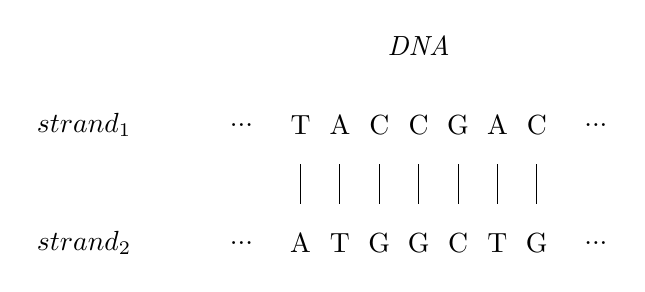
\begin{tikzpicture}
  % texts
  \node at(2.25,2.5)(title){\textit{DNA}};
  \node at(-2,0)(title){\textit{$strand_2$}};
  \node at(-2,1.5)(title){\textit{$strand_1$}};
  % lower nodes
  \node at(0,0)(n1){...};
  \node at(.75,0)(n2){A};
  \node at(1.25,0)(n3){T};
  \node at(1.75, 0)(n4){G};
  \node at(2.25,0)(n5){G};
  \node at(2.75,0)(n5){C};
  \node at(3.25,0)(n5){T};
  \node at(3.75,0)(n5){G};
  \node at(4.5,0)(n5){...};
  % upper nodes
  \node at(0,1.5)(n1){...};
  \node at(.75,1.5)(n2){T};
  \node at(1.25,1.5)(n3){A};
  \node at(1.75,1.5)(n4){C};
  \node at(2.25,1.5)(n5){C};
  \node at(2.75,1.5)(n5){G};
  \node at(3.25,1.5)(n5){A};
  \node at(3.75,1.5)(n5){C};
  \node at(4.5,1.5)(n5){...};
  % base pair bonds 
  \draw (.75,.5) -- (.75,1);
  \draw (1.25,.5) -- (1.25,1);
  \draw (1.75,.5) -- (1.75,1);
  \draw (2.25,.5) -- (2.25,1);
  \draw (2.75,.5) -- (2.75,1);
  \draw (3.25,.5) -- (3.25,1);
  \draw (3.75,.5) -- (3.75,1);
\end{tikzpicture}
}
\caption{A conceptual representation of a DNA molecule made up of two strands. The strands are composed of nucleotides forming base pairs where A (adenine) and T (thymine), and C (cytosine) and G (guanine) are complements of each other.}
\label{background:biology:dna_and_chromosomes:figures:dna_strands}
\end{center}
\end{figure}

Relatively small differences in these DNA sequences are what differentiates individuals within the same species from one other.
It is therefore interesting to study these sequences of nucleotides encoding organisms' genetic information, as the encoded information can reveal details about both associated physical traits and diseases.
In human cells, these DNA strands are estimated to be roughly $3 * 10^{9}$ bases long \cite[p.13]{singh}.

DNA is organized into structures called \textit{chromosomes}. 
Humans have 23 chromosome pairs, making up a total of 46 chromosomes.
Each of the pairs include one version of the chromosome inherited from the male parent, and one version inherited from the female parent \cite{nhgri_chromosome}.

The term \textit{genome} can be used to refer to the complete genetic material of an organism.
In practice, however, the genome of an organism often simply refers to the complete DNA nucleotide sequence of one set of chromosomes for that organism \cite[p.13]{singh}.
Commonly in bioinformatics, one can also encounter the term \textit{reference genome}, referring to a theoretical reconstruction of an organism's genome created by scientists.
Such genome reconstructions are commonly used when examining new DNA sequences, often by aligning new DNA sequences to the reference in order to see at which positions their nucleotides differ and what differences are present at those positions \cite{gatk}.

